% Options for packages loaded elsewhere
\PassOptionsToPackage{unicode}{hyperref}
\PassOptionsToPackage{hyphens}{url}
%
\documentclass[
  american,
]{article}
\usepackage{lmodern}
\usepackage{amsmath}
\usepackage{ifxetex,ifluatex}
\ifnum 0\ifxetex 1\fi\ifluatex 1\fi=0 % if pdftex
  \usepackage[T1]{fontenc}
  \usepackage[utf8]{inputenc}
  \usepackage{textcomp} % provide euro and other symbols
  \usepackage{amssymb}
\else % if luatex or xetex
  \usepackage{unicode-math}
  \defaultfontfeatures{Scale=MatchLowercase}
  \defaultfontfeatures[\rmfamily]{Ligatures=TeX,Scale=1}
  \setmainfont{LinLibertineO}
  \setsansfont{Carlito}
  \setmonofont{DejaVuSansMono}
\fi
% Use upquote if available, for straight quotes in verbatim environments
\IfFileExists{upquote.sty}{\usepackage{upquote}}{}
\IfFileExists{microtype.sty}{% use microtype if available
  \usepackage[]{microtype}
  \UseMicrotypeSet[protrusion]{basicmath} % disable protrusion for tt fonts
}{}
\makeatletter
\@ifundefined{KOMAClassName}{% if non-KOMA class
  \IfFileExists{parskip.sty}{%
    \usepackage{parskip}
  }{% else
    \setlength{\parindent}{0pt}
    \setlength{\parskip}{6pt plus 2pt minus 1pt}}
}{% if KOMA class
  \KOMAoptions{parskip=half}}
\makeatother
\usepackage{xcolor}
\IfFileExists{xurl.sty}{\usepackage{xurl}}{} % add URL line breaks if available
\IfFileExists{bookmark.sty}{\usepackage{bookmark}}{\usepackage{hyperref}}
\hypersetup{
  pdftitle={FeenoX Software Design Specification},
  pdflang={en-US},
  hidelinks,
  pdfcreator={LaTeX via pandoc}}
% \urlstyle{same} % disable monospaced font for URLs
\usepackage{graphicx}
\makeatletter
\def\maxwidth{\ifdim\Gin@nat@width>\linewidth\linewidth\else\Gin@nat@width\fi}
\def\maxheight{\ifdim\Gin@nat@height>\textheight\textheight\else\Gin@nat@height\fi}
\makeatother
% Scale images if necessary, so that they will not overflow the page
% margins by default, and it is still possible to overwrite the defaults
% using explicit options in \includegraphics[width, height, ...]{}
\setkeys{Gin}{width=\maxwidth,height=\maxheight,keepaspectratio}
% Set default figure placement to htbp
\makeatletter
\def\fps@figure{htbp}
\makeatother
% headers y footers a medida
\usepackage{lastpage}
\usepackage{fancyhdr}
\pagestyle{fancy}
\fancyhf{} % clear all header and footer fields
\lhead{FeenoX Software Design Specification}
\lfoot{\scriptsize{ / }}
\rfoot{\thepage/\pageref{LastPage}}
\rhead{
\includegraphics[height=10pt]{logo}}
\renewcommand{\headrulewidth}{0.0pt}
\renewcommand{\footrulewidth}{0.4pt}

\fancypagestyle{plain}{%
\fancyhf{} % clear all header and footer fields
\renewcommand{\headrulewidth}{0pt}
\renewcommand{\footrulewidth}{0pt}}

\setlength{\emergencystretch}{3em} % prevent overfull lines
\providecommand{\tightlist}{%
  \setlength{\itemsep}{0pt}\setlength{\parskip}{0pt}}
\setcounter{secnumdepth}{5}
\makeatletter
\@ifpackageloaded{subfig}{}{\usepackage{subfig}}
\@ifpackageloaded{caption}{}{\usepackage{caption}}
\captionsetup[subfloat]{margin=0.5em}
\AtBeginDocument{%
\renewcommand*\figurename{Figure}
\renewcommand*\tablename{Table}
}
\AtBeginDocument{%
\renewcommand*\listfigurename{List of Figures}
\renewcommand*\listtablename{List of Tables}
}
\@ifpackageloaded{float}{}{\usepackage{float}}
\floatstyle{ruled}
\@ifundefined{c@chapter}{\newfloat{codelisting}{h}{lop}}{\newfloat{codelisting}{h}{lop}[chapter]}
\floatname{codelisting}{Listing}
\newcommand*\listoflistings{\listof{codelisting}{List of Listings}}
\makeatother
\ifxetex
  % Load polyglossia as late as possible: uses bidi with RTL langages (e.g. Hebrew, Arabic)
  \usepackage{polyglossia}
  \setmainlanguage[variant=american]{english}
\else
  \usepackage[shorthands=off,main=american]{babel}
\fi
\ifluatex
  \usepackage{selnolig}  % disable illegal ligatures
\fi

\lstdefinelanguage{feenox}{
morekeywords={
      ABORT,
      ALIAS,
      ALLOW_NEW_NONZEROS,
      ALLOW_UNRESOLVED_BCS,
      APPEND,
      AS,
      ASCENDING,
      ASCENDING_ORDER,
      ASCII_FILE,
      ASCII_FILE_PATH,
      AXISYMMETRIC,
      BC,
      BINARY_FILE,
      BINARY_FILE_PATH,
      BOUNDARY_CONDITION,
      CACHE_B,
      CACHE_J,
      CELL,
      CELLS,
      CLOSE,
      COLS,
      COLUMNS,
      COMPUTE_REACTION,
      DATA,
      DEFAULT_ARGUMENT_VALUE,
      DESCENDING,
      DESCENDING_ORDER,
      DETECT_HANGING_NODES,
      DETECT_UNRESOLVED_BCS,
      DIM,
      DIMENSION,
      DIMENSIONS,
      DIRICHLET_SCALING,
      DUMP,
      EIGEN_DIRICHLET_ZERO,
      EIGEN_FORMULATION,
      EIGEN_SOLVER,
      ELSE,
      ENDIF,
      EPS,
      EPSABS,
      EPSREL,
      EPS_TYPE,
      FILE,
      FILE_FORMAT,
      FILE_PATH,
      FIND_EXTREMA,
      FIT,
      FOR,
      FORMAT,
      FROM,
      FUNCTION,
      FUNCTION_DATA,
      GAUSS,
      GRADIENT,
      GROUP,
      GROUPS,
      HANDLE_HANGING_NODES,
      HEADER,
      HISTORY,
      ID,
      IF,
      IGNORE_NULL,
      I_MAX,
      I_MIN,
      IMPLICIT,
      INCLUDE,
      INITIAL_CONDITIONS,
      INITIAL_CONDITIONS_MODE,
      INPUT,
      INPUT_FILE,
      INTEGRATE,
      INTEGRATION,
      INTERPOLATION,
      INTERPOLATION_THRESHOLD,
      IS,
      K,
      K_bc,
      KSP,
      KSP_TYPE,
      LABEL,
      LINEAR,
      LINEARIZE_STRESS,
      LINEAR_SOLVER,
      M,
      MAIN,
      MATERIAL,
      MATRIX,
      MAX,
      MAX_ITER,
      M_bc,
      MESH,
      METHOD,
      MIN,
      MODE,
      MODES,
      MOMENT,
      N,
      NAME,
      NODE,
      NODES,
      NO_MESH,
      NOMESH,
      NONEWLINE,
      NON_LINEAR,
      NON_LINEAR_SOLVER,
      NONLINEAR_SOLVER,
      NO_PHYSICAL_NAMES,
      NSTEPS,
      OFFSET,
      OPEN,
      OUTPUT,
      OUTPUT_FILE,
      OVER,
      PATH,
      PC,
      PC_TYPE,
      PETSC_OPTIONS,
      PHASE_SPACE,
      PHYSICAL_ENTITY,
      PHYSICAL_GROUP,
      PREALLOCATE,
      PRECONDITIONER,
      PRINT,
      PRINTF,
      PRINTF_ALL,
      PRINT_FUNCTION,
      PRINT_VECTOR,
      PROBLEM,
      PROGRESS,
      PROGRESS_ASCII,
      QUASISTATIC,
      RANGE_MAX,
      RANGE_MIN,
      REACTION,
      READ,
      READ_FIELD,
      READ_FUNCTION,
      READ_MESH,
      READ_SYMMETRIC_TENSOR,
      READ_VECTOR,
      RE_READ,
      RESULT,
      ROWS,
      SCALE,
      SEM,
      SEMAPHORE,
      SEP,
      SEPARATOR,
      SHEPARD_EXPONENT,
      SHEPARD_RADIUS,
      SHM,
      SHM_OBJECT,
      SIZE,
      SIZES,
      SN,
      SNES,
      SNES_TYPE,
      SOLVE,
      SOLVE_PROBLEM,
      SORT_VECTOR,
      SPECTRAL_TRANSFORMATION,
      ST,
      STEP,
      STRING,
      ST_TYPE,
      SYMMETRIC_TENSOR,
      SYMM_TENSOR,
      TEXT,
      TIME_ADAPTATION,
      TIME_PATH,
      TO,
      TOL_ABS,
      TOL_REL,
      TRANSIENT,
      TRANSIENT_SOLVER,
      TS,
      TS_ADAPT,
      TS_ADAPT_TYPE,
      TS_TYPE,
      UNKNOWNS,
      UPDATE_EACH_STEP,
      VAR,
      VARIABLE,
      VARIABLES,
      VARS,
      VECTOR,
      VECTORS,
      VECTOR_SORT,
      VERBOSE,
      VIA,
      WRITE,
      WRITE_MESH,
      WRITE_RESULTS,
      X0,
      X_INCREASES_FIRST,
      X_MAX,
      X_MIN,
      Y0,
      Y_MAX,
      Y_MIN,
      Z0,
      Z_MAX,
      Z_MIN,
      ALLOWED,
      AS_PROVIDED,
      K,
      M,
      NONE,
      POST,
      SKIP_HEADER_STEP,
      SKIP_STATIC_STEP,
      SKIP_STEP,
      SKIP_TIME,
      WAIT,
},
morekeywords={[2]$
},
morekeywords={[3]
      alpha,
      alpha_0,
      alpha_x,
      alpha_x_0,
      alphax,
      alphax_0,
      alpha_y,
      alpha_y_0,
      alphay,
      alphay_0,
      alpha_z,
      alpha_z_0,
      alphaz,
      alphaz_0,
      cp,
      cp_0,
      dae_rtol,
      dae_rtol_0,
      delta_sigma_max,
      delta_sigma_max_0,
      displ_max,
      displ_max_0,
      displ_max_x,
      displ_max_x_0,
      displ_max_y,
      displ_max_y_0,
      displ_max_z,
      displ_max_z_0,
      done,
      done_0,
      done_static,
      done_static_0,
      done_transient,
      done_transient_0,
      dont_quit,
      dont_quit_0,
      dont_report,
      dont_report_0,
      dt,
      dt_0,
      E,
      E_0,
      end_time,
      end_time_0,
      eps_max_it,
      eps_max_it_0,
      eps_st_nu,
      eps_st_nu_0,
      eps_st_sigma,
      eps_st_sigma_0,
      eps_tol,
      eps_tol_0,
      E_x,
      E_x_0,
      Ex,
      Ex_0,
      E_y,
      E_y_0,
      Ey,
      Ey_0,
      E_z,
      E_z_0,
      Ez,
      Ez_0,
      f_x,
      f_x_0,
      fx,
      fx_0,
      f_y,
      f_y_0,
      fy,
      fy_0,
      f_z,
      f_z_0,
      fz,
      fz_0,
      gamg_threshold,
      gamg_threshold_0,
      G_xy,
      G_xy_0,
      Gxy,
      Gxy_0,
      G_yz,
      G_yz_0,
      Gyz,
      Gyz_0,
      G_zx,
      G_zx_0,
      Gzx,
      Gzx_0,
      i,
      i_0,
      infinite,
      infinite_0,
      in_static,
      in_static_0,
      in_static_first,
      in_static_first_0,
      in_static_last,
      in_static_last_0,
      in_transient,
      in_transient_0,
      in_transient_first,
      in_transient_first_0,
      in_transient_last,
      in_transient_last_0,
      j,
      j_0,
      k,
      k_0,
      kappa,
      kappa_0,
      keff,
      keff_0,
      ksp_atol,
      ksp_atol_0,
      ksp_divtol,
      ksp_divtol_0,
      ksp_max_it,
      ksp_max_it_0,
      ksp_rtol,
      ksp_rtol_0,
      max_dt,
      max_dt_0,
      memory_available,
      memory_available_0,
      min_dt,
      min_dt_0,
      mpi_rank,
      mpi_rank_0,
      mpi_size,
      mpi_size_0,
      mumps_icntl_14,
      mumps_icntl_14_0,
      nodes_rough,
      nodes_rough_0,
      nu,
      nu_0,
      nu_xy,
      nu_xy_0,
      nuxy,
      nuxy_0,
      nu_yz,
      nu_yz_0,
      nuyz,
      nuyz_0,
      nu_zx,
      nu_zx_0,
      nuzx,
      nuzx_0,
      on_gsl_error,
      on_gsl_error_0,
      on_nan,
      on_nan_0,
      on_sundials_error,
      on_sundials_error_0,
      penalty_weight,
      penalty_weight_0,
      pi,
      pi_0,
      pid,
      pid_0,
      q,
      q_0,
      q''',
      q'''_0,
      quit,
      quit_0,
      realtime_scale,
      realtime_scale_0,
      report,
      report_0,
      rho,
      rho_0,
      rhocp,
      rhocp_0,
      sigma_max,
      sigma_max_0,
      sigma_max_x,
      sigma_max_x_0,
      sigma_max_y,
      sigma_max_y_0,
      sigma_max_z,
      sigma_max_z_0,
      sn_alpha,
      sn_alpha_0,
      snes_atol,
      snes_atol_0,
      snes_max_it,
      snes_max_it_0,
      snes_rtol,
      snes_rtol_0,
      snes_stol,
      snes_stol_0,
      static_steps,
      static_steps_0,
      step_static,
      step_static_0,
      step_transient,
      step_transient_0,
      strain_energy,
      strain_energy_0,
      t,
      t_0,
      T,
      T_0,
      T_0,
      T_0_0,
      T0,
      T0_0,
      T_guess,
      T_guess_0,
      thermal,
      thermal_0,
      conductivity,
      conductivity_0,
      T_max,
      T_max_0,
      T_min,
      T_min_0,
      total_dofs,
      total_dofs_0,
      ts_atol,
      ts_atol_0,
      ts_rtol,
      ts_rtol_0,
      U,
      U_0,
      u_at_displ_max,
      u_at_displ_max_0,
      u_at_sigma_max,
      u_at_sigma_max_0,
      V,
      V_0,
      v_at_displ_max,
      v_at_displ_max_0,
      v_at_sigma_max,
      v_at_sigma_max_0,
      W,
      W_0,
      w_at_displ_max,
      w_at_displ_max_0,
      w_at_sigma_max,
      w_at_sigma_max_0,
      x,
      x_0,
      y,
      y_0,
      z,
      z_0,
      zero,
      zero_0,
},
morekeywords={[4]
      abs,
      acos,
      asin,
      atan,
      atan2,
      ceil,
      clock,
      cos,
      cosh,
      cpu_time,
      d_dt,
      deadband,
      derivative,
      equal,
      exp,
      expint1,
      expint2,
      expint3,
      expintn,
      floor,
      func_min,
      gammaf,
      gauss_kronrod,
      gauss_legendre,
      heaviside,
      if,
      integral,
      integral_dt,
      integral_euler_dt,
      is_even,
      is_in_interval,
      is_odd,
      j0,
      lag,
      lag_bilinear,
      lag_euler,
      last,
      limit,
      limit_dt,
      log,
      mark_max,
      mark_min,
      max,
      memory,
      min,
      mod,
      mpi_memory_global,
      mpi_memory_local,
      not,
      prod,
      qrng2d_halton,
      qrng2d_niederreiter,
      qrng2d_reversehalton,
      qrng2d_sobol,
      qrng_halton,
      qrng_niederreiter,
      qrng_reversehalton,
      qrng_sobol,
      quasi_random,
      random,
      random_gauss,
      root,
      round,
      sawtooth_wave,
      sech,
      sgn,
      sin,
      sinh,
      sqrt,
      square_wave,
      sum,
      tan,
      tanh,
      threshold_max,
      threshold_min,
      triangular_wave,
      vecdot,
      vecmax,
      vecmaxindex,
      vecmin,
      vecminindex,
      vecnorm,
      vecsize,
      vecsum,
      wall_time,
},
sensitive=true,
morecomment=[l]{\#},
morestring=[b]\",
}


\definecolor{was_keyword1}{rgb}{0.0,0.0,0.4}
\definecolor{was_keyword2}{rgb}{0.0,0.2,0.0}
\definecolor{was_variable}{rgb}{0.5,0.2,0.2}
\definecolor{was_function}{rgb}{0.2,0.5,0.2}
\definecolor{was_comment}{rgb}{0.5,0.5,0.5}

\definecolor{bash_keyword1}{rgb}{0.2,0.2,0.2}
\definecolor{bash_keyword2}{rgb}{0.7,0.7,0.7}
\definecolor{bash_comment}{rgb}{0.5,0.5,0.5}

\definecolor{python_keyword2}{rgb}{0.5,0.2,0.8}

\definecolor{was_fondo}{rgb}{0.95,0.95,0.90}
\definecolor{fino_fondo}{rgb}{0.90,0.95,0.90}
\definecolor{gmsh_fondo}{rgb}{0.90,0.90,0.95}
\definecolor{terminal_fondo}{rgb}{0.2,0.2,0.2}
\definecolor{awk_fondo}{rgb}{0.95,0.90,0.95}
\definecolor{bash_fondo}{rgb}{0.90,0.90,0.90}

\definecolor{terminal_fore}{rgb}{1.0,1.0,1.0}


\newcommand{\MyHookSign}{\hbox{\ensuremath{\hookleftarrow}}}

% default
\lstset{
  basicstyle=\ttfamily\footnotesize,
  backgroundcolor=\color{bash_fondo},
  breaklines=true,
  prebreak={\space\MyHookSign},
  xleftmargin=0.2cm,
  xrightmargin=0.2cm,
  framesep=0.2cm,
  frame=single,
}


\lstdefinestyle{feenox}{
  language=feenox,
  basicstyle=\ttfamily\footnotesize,
  commentstyle={\color{was_comment}\normalfont\textit},
  keywordstyle=[1]{\color{was_keyword1}\ttfamily\textbf},
  keywordstyle=[2]{\color{was_keyword2}\ttfamily\textbf},
  keywordstyle=[3]{\color{was_variable}\textit},
  keywordstyle=[4]{\color{was_function}\textbf},
  backgroundcolor=\color{was_fondo},
  showstringspaces=true,
  breaklines=true,
  breakatwhitespace=true,
  prebreak={\space\MyHookSign},
  lineskip=-1pt,
  captionpos=b,
%   numbers=left,
%   stepnumber=5,
  xleftmargin=0.2cm,
  xrightmargin=0.4cm,
  framesep=0.1cm,
  frame=single,
}


\lstdefinestyle{bash}{
  language=bash,
  basicstyle=\ttfamily\footnotesize,
  commentstyle={\color{bash_comment}\normalfont\textit},
  keywordstyle=[1]{\color{bash_keyword1}\ttfamily\textbf},
  keywordstyle=[2]{\color{bash_keyword2}\ttfamily\textbf},
  backgroundcolor=\color{bash_fondo},
  showstringspaces=true,
  breaklines=true,
  breakatwhitespace=true,
  prebreak={\space\MyHookSign},
  lineskip=-1pt,
  captionpos=b,
%   numbers=left,
%   stepnumber=5,
  xleftmargin=0.2cm,
  xrightmargin=0.2cm,
  framesep=0.2cm,
  frame=single,
}


\lstdefinestyle{terminal}{
  language=,
  basicstyle=\ttfamily\footnotesize\color{terminal_fore},
  backgroundcolor=\color{terminal_fondo},
  breaklines=true,
  prebreak={\space\MyHookSign},
  xleftmargin=0.2cm,
  xrightmargin=0.2cm,
  framesep=0.2cm,
  frame=single,
}

\lstdefinestyle{c}{
  language=C,
  basicstyle=\ttfamily\footnotesize,                                
  commentstyle={\color{was_comment}\normalfont\textit},     
  keywordstyle=[1]{\color{was_keyword1}\ttfamily\textbf},   
  keywordstyle=[2]{\color{was_keyword2}\ttfamily\textbf},   
  keywordstyle=[3]{\color{was_variable}\textit},            
  keywordstyle=[4]{\color{was_function}\textbf},            
  backgroundcolor=\color{gmsh_fondo},                       
  showstringspaces=true,                                    
  breaklines=true,                                          
  breakatwhitespace=true,                                   
  prebreak={\space\MyHookSign},                             
  lineskip=-1pt,                                            
  captionpos=b,
%   numbers=left,
%   stepnumber=5,
  xleftmargin=0.2cm,                                        
  xrightmargin=0.4cm,                                       
  framesep=0.1cm,                                           
  frame=single,                                             
}

\lstdefinestyle{cpp}{
  language=C++,
  basicstyle=\ttfamily\footnotesize,                                
  commentstyle={\color{was_comment}\normalfont\textit},     
  keywordstyle=[1]{\color{was_keyword1}\ttfamily\textbf},   
  keywordstyle=[2]{\color{was_keyword2}\ttfamily\textbf},   
  keywordstyle=[3]{\color{was_variable}\textit},            
  keywordstyle=[4]{\color{was_function}\textbf},            
  backgroundcolor=\color{gmsh_fondo},                       
  showstringspaces=true,                                    
  breaklines=true,                                          
  breakatwhitespace=true,                                   
  prebreak={\space\MyHookSign},                             
  lineskip=-1pt,                                            
  captionpos=b,
%   numbers=left,
%   stepnumber=5,
  xleftmargin=0.2cm,                                        
  xrightmargin=0.4cm,                                       
  framesep=0.1cm,                                           
  frame=single,                                             
}




\lstdefinestyle{awk}{
  language=awk,
  basicstyle=\ttfamily\footnotesize,                                
  commentstyle={\color{was_comment}\normalfont\textit},     
  keywordstyle=[1]{\color{was_keyword1}\ttfamily\textbf},   
  keywordstyle=[2]{\color{was_keyword2}\ttfamily\textbf},   
  keywordstyle=[3]{\color{was_variable}\textit},            
  keywordstyle=[4]{\color{was_function}\textbf},            
  backgroundcolor=\color{awk_fondo},                       
  showstringspaces=true,                                    
  breaklines=true,                                          
  breakatwhitespace=true,                                   
  prebreak={\space\MyHookSign},                             
  lineskip=-1pt,                                            
  captionpos=b,
%   numbers=left,
%   stepnumber=5,
  xleftmargin=0.2cm,                                        
  xrightmargin=0.4cm,                                       
  framesep=0.1cm,                                           
  frame=single,                                             
}

\lstdefinestyle{python}{
  language=python,
  basicstyle=\ttfamily\footnotesize,
  commentstyle={\color{bash_comment}\normalfont\textit},
  keywordstyle=[1]{\color{bash_keyword1}\ttfamily\textbf},
  keywordstyle=[2]{\color{python_keyword2}\ttfamily\textbf},
  backgroundcolor=\color{awk_fondo},
  showstringspaces=true,
  breaklines=true,
  breakatwhitespace=true,
  prebreak={\space\MyHookSign},
  lineskip=-1pt,
  captionpos=b,
%   numbers=left,
%   stepnumber=5,
  xleftmargin=0.1cm,
  xrightmargin=0.1cm,
  framesep=0.1cm,
  frame=single,
}


\usepackage{subfig}
% SIunits
\usepackage{siunitx}

% fuente para los captions de figuras
\usepackage{caption}
\renewcommand{\captionfont}{\sf\small}
% \renewcommand{\captionlabelfont}{\bf\sf}

\title{FeenoX Software Design Specification}
\author{}
\date{}

\begin{document}
% \thispagestyle{empty}
% \thispagestyle{plain}
% \thispagestyle{fancy}

\maketitle
\begin{abstract}
This design specification addresses the (hypothetical) Software
Requirement Specification for developing a piece of free and open source
engineering software with certain specifications, defined in an
imaginary tender.
\end{abstract}


% vectors done right
\renewcommand{\vec}[1]{\ensuremath\mathbf{#1}}

\hypertarget{sec:introduction}{%
\section{Introduction}\label{sec:introduction}}

\begin{quote}
A cloud-based computational tool (herein after referred to as \emph{the
tool}) is required in order to solve engineering problems following the
current state-of-the-art methods and technologies impacting the
high-performance computing world. This (imaginary but plausible)
Software Requirements Specification document describes the mandatory
features this tool ought to have and lists some features which would be
nice the tool had. Also it contains requirements and guidelines about
architecture, execution and interfaces in order to fulfill the needs of
cognizant engineers as of 2021 (and the years to come) are defined.

On the one hand, the tool should be applicable to solving industrial
problems under stringent efficiency (sec.~\ref{sec:efficiency}) and
quality (sec.~\ref{sec:qa}) requirements. It is therefore mandatory to
be able to assess the source code for potential performance and
verification revision by qualified third parties from all around the
world. On the other hand, the initial version of the tool is expected to
be a basic framework which might be extended (sec.~\ref{sec:objective}
and sec.~\ref{sec:extensibility}) by academic researchers and
programmers. It thus should also be free.\footnote{Free as in ``free
  speech,'' not as in ``free beer.''} The detailed licensing terms are
left to the offer but it should allow users to solve their problems the
way they need and, eventually, to modify and improve the tool to suit
their needs. If they cannot program themselves, they should have the
freedom to hire somebody to do it for them.
\end{quote}

Besides noting that software being \emph{free} (regarding freedom, not
price) does not imply the same as being \emph{open source}, the
requirement is clear in that the tool has to be both \emph{free} and
\emph{open source}, a combination which is usually called
\href{https://en.wikipedia.org/wiki/Free_and_open-source_software}{FOSS}.
This condition leaves all of the well-known non-free finite-element
solvers in the market out of the tender.

FeenoX is licensed under the terms of the
\href{https://www.gnu.org/licenses/gpl-3.0}{GNU General Public License}
version~3 or, at the user convenience, any later version. This means
that users get the four essential freedoms:

\begin{enumerate}
\def\labelenumi{\arabic{enumi}.}
\setcounter{enumi}{-1}
\tightlist
\item
  The freedom to \emph{run} the program as they wish, for \emph{any}
  purpose.
\item
  The freedom to \emph{study} how the program works, and \emph{change}
  it so it does their computing as they wish.
\item
  The freedom to \emph{redistribute} copies so they can help others.
\item
  The freedom to \emph{distribute} copies of their \emph{modified}
  versions to others.
\end{enumerate}

There are some examples of pieces of computational software which are
described as ``open source'' in which even the first of the four
freedoms is denied. The most iconic case is that of Android, whose
sources are readily available online but there is no straightforward way
of updating one's mobile phone firmware with a customized version, not
to mention vendor and hardware lock ins and the possibility of bricking
devices if something unexpected happens. In the nuclear industry, it is
the case of a Monte Carlo particle-transport program that requests users
to sign an agreement about the objective of its usage before allowing
its execution. The software itself might be open source because the
source code is provided after signing the agreement, but it is not free
(as in freedom) at all.

So a free program has to be open source, but it also has to explicitly
provide the four freedoms above both through the written license and
through the mechanisms available to get, modify, compile, run and
document these modifications. That is why licensing FeenoX as GPLv3+
also implies that the source code and all the scripts and makefiles
needed to compile and run it are available for anyone that requires it.
Anyone wanting to modify the program either to fix bugs, improve it or
add new features is free to do so. And if they do not know how to
program, the have the freedom to hire a programmer to do it without
needing to ask permission to the original authors.

Nevertheless, since these original authors are the copyright holders,
they still can use it to either enforce or prevent further actions from
the users that receive FeenoX under the GPLv3+. In particular, the
license allows re-distribution of modified versions only if they are
clearly marked as different from the original and only under the same
terms of the GPLv3+. There are also some other subtle technicalities
that need not be discussed here such as what constitutes a modified
version (which cannot be redistributed under a different license) and
what is an aggregate (in which each part be distributed under different
licenses) and about usage over a network and the possibility of using
\href{https://en.wikipedia.org/wiki/GNU_Affero_General_Public_License}{AGPL}
instead of GPL to further enforce freedom (TLDR; it does not matter for
FeenoX), but which are already taken into account in FeenoX licensing
scheme.

\hypertarget{sec:objective}{%
\subsection{Objective}\label{sec:objective}}

\begin{quote}
The main objective of the tool is to be able to solve engineering
problems which are usually casted as differential-algebraic equations
(DAEs) or partial differential equations (PDEs), such as

\begin{itemize}
\tightlist
\item
  dynamical systems
\item
  plant control dynamics
\item
  mechanical elasticity
\item
  heat conduction
\item
  structural modal analysis
\item
  electromagnetism
\item
  chemical diffusion
\item
  computational fluid dynamics
\item
  \ldots{}
\end{itemize}

on one or more manistream cloud servers, i.e.~computers with an
architecture (i.e.~hardware and operating systems, futher discussed in
sec.~\ref{sec:architecture}) that allows them to be available online and
accessed remotely either interactively or automatically by other
computers as well. Other architectures such as high-end desktop personal
computers or even low-end laptops might be supported but they should not
the main target.

The initial version of the tool must be able to handle a subset of the
above list of problem types. Afterward, the set of supported problem
types, models, equations and features of the tool should grow to include
other models as well, as required in~sec.~\ref{sec:extensibility}.
\end{quote}

The choice of the initial supported features is based on the types of
problem that the FeenoX' precursor codes (namely wasora, Fino and
milonga) already have been supporting since more than ten years now. It
is also a first choice so work can be bounded and a subsequent road map
and release plans can be designed. FeenoX' first version includes a
subset of the required functionality, namely

\begin{itemize}
\tightlist
\item
  dynamical systems
\item
  plant control dynamics
\item
  heat conduction
\item
  mechanical elasticity
\item
  structural modal analysis
\item
  multigroup neutron transport and diffusion
\end{itemize}

FeenoX is designed to be developed and executed under GNU/Linux, which
is the architecture og more than 95\% of the internet servers which we
collectively call ``the cloud.'' It should be noted that GNU/Linux is a
POSIX-compliant version of UNIX and that FeenoX follows the rules of
UNIX philosophy (sec.~\ref{sec:unix}) regarding its computational
implementation code. Besides POSIX, FeenoX also uses MPI which is a
well-known industry standard for massive parallel executions of
processes, both in multi-core hosts and multi-hosts environments.
Finally, if performance and/or scalability are not important issues,
FeenoX can be run in a (properly cooled) local PC or laptop.

The requirement to run in the cloud and scale up as needed rules out
some of the FOSS solvers available online, such as CalculiX.

\hypertarget{sec:scope}{%
\subsection{Scope}\label{sec:scope}}

\begin{quote}
The tool should allow advanced users to define the problem to be solved
programmatically, using one or more files either\ldots{}

\begin{enumerate}
\def\labelenumi{\alph{enumi}.}
\tightlist
\item
  specifically formatted for the tool to read such as JSON or a
  particular input format (historically called input decks in
  punched-card days), and/or
\item
  written in an high-level interpreted language such as Python or Julia.
\end{enumerate}

It should be noted that a graphical user interface is not required. The
tool may include one, but it should be able to run without needing any
user intervention rather than the preparation of a set of input files.
Nevertheless, there tool might \emph{allow} a GUI to be used. For
example, for a basic usage involving simple cases, a user interface
engine should be able to create these problem-definition files in order
to give access to less advanced users to the tool using a desktop,
mobile and/or web-based interface in order to run the actual tool
without further intervention.

However, for general usage, users should be able to completely define
the problem (or set of problems, i.e.~a parametric study) they want to
solve in one or more input files and to obtain one or more output files
containing the desired results, either a set of scalar outputs (such as
maximum stresses or mean temperatures), and/or a time and/or spatial
distribution. If needed, a discretization of the domain may to be taken
as a know input, i.e.~the tool is not required to create the mesh as
long as a suitable mesher can be employed using a similar workflow
specified in this~SRS.

The tool should define and document (sec.~\ref{sec:documentation}) the
way the input files for a solving particular problem are to be prepared
(sec.~\ref{sec:input}) and how the results are to be written
(sec.~\ref{sec:output}). Any GUI, pre-processor, post-processor or other
related graphical tool used to provide a graphical interface for the
user should integrate in the workflow described in the preceding
paragraph: a pre-processor should create the input files needed for the
tool and a post-processor should read the output files created by the
tool.
\end{quote}

Indeed, FeenoX is designed to work very much like a transfer function
between two (or more) files---usually the FeenoX input file and the
problem mesh file---and zero or more output files---usually the terminal
output and a VTK post-processing file---as illustrated in
fig.~\ref{fig:transfer}.

\begin{figure}
\hypertarget{fig:transfer}{%
\centering

\includegraphics[width=0.5\textwidth,height=\textheight]{transfer.svg}
\caption{FeenoX working as a transfer function between input and output
files}\label{fig:transfer}
}
\end{figure}

In some particular cases, FeenoX can also provide an API for high-level
interpreted languages such as Python or Julia such that a problem can be
completely defined in a script, increasing also flexibility.

As already stated, FeenoX is designed and implemented following the UNIX
philosophy in general and Eric Raymond's 17 Unix Rules ({[}sec:unix{]})
in particular. One of the main ideas is the rule of \emph{separation}
that essentially implies to separate mechanism from policy, that in the
computational engineering world translates into separating the frontend
from the backend. Even though most FEA programs eventually separate the
interface from the solver up to some degree, there are cases in which
they are still dependent such that changing the former needs updating
the latter.

From the very beginning, FeenoX is designed as a pure backend which
should nevertheless provide appropriate mechanisms for different
frontends to be able to communicate and to provide a friendly interface
for the final user. Yet, the separation is complete in the sense that
the nature of the frontends can radically change (say from a
desktop-based point-and-click program to a web-based immersive
augmented-reality application) without needing the modify the backend.
Not only far more flexibility is given by following this path, but also
develop efficiency and quality is encouraged since programmers working
on the lower-level of an engineering tool usually do not have the skills
needed to write good user-experience interfaces, and conversely.

In the very same sense, FeenoX does not discretize continuous domains
for PDE problems itself, but relies on separate tools for this end.
Fortunately, there already exists one meshing tool which is FOSS (GPLv2)
and shares most (if not all) of the design basis principles with FeenoX:
the three-dimensional finite element mesh generator
\href{http://gmsh.info/}{Gmsh}. Strictly speaking, FeenoX does not need
to be used along with Gmsh but with any other mesher able to write
meshes in Gmsh's format \passthrough{\lstinline!.msh!}. But since Gmsh
also

\begin{itemize}
\tightlist
\item
  is free and open source,
\item
  works also in a transfer-function-like fashion,
\item
  runs natively on GNU/Linux,
\item
  has a similar (but more comprehensive) API for Python/Julia,
\item
  etc.
\end{itemize}

\noindent it is a perfect match for FeenoX. Even more, it provides
suitable domain decomposition methods (through other FOSS third-party
libraries such as
\href{http://glaros.dtc.umn.edu/gkhome/metis/metis/overview}{Metis}) for
scaling up large problems,

For example, the famous chaotic
\href{http://en.wikipedia.org/wiki/Lorenz_system}{Lorenz' dynamical
system}---the one of the butterfly---whose differential equations are

\begin{equation*}
\begin{cases}
\dot{x} &= \sigma \cdot (y - x)  \\
\dot{y} &= x \cdot (r - z) - y   \\
\dot{z} &= x y - b z       \\
\end{cases}
\end{equation*}

where \(\sigma=10\), \(b=8/3\) and \(r=28\) are the classical parameters
that generate the butterfly as presented by Edward Lorenz back in his
seminal 1963 paper
\href{http://journals.ametsoc.org/doi/abs/10.1175/1520-0469\%281963\%29020\%3C0130\%3ADNF\%3E2.0.CO\%3B2}{Deterministic
non-periodic flow}, can be solved with FeenoX by writing the equations
in the input file as naturally as possible, as illustrated in the input
file that follows:

\begin{lstlisting}[style=feenox]
PHASE_SPACE x y z     # Lorenz attractor’s phase space is x-y-z
end_time = 40         # we go from t=0 to 40 non-dimensional units

sigma = 10            # the original parameters from the 1963 paper
r = 28
b = 8/3

x_0 = -11             # initial conditions
y_0 = -16
z_0 = 22.5

# the dynamical system's equations written as naturally as possible
x_dot .= sigma*(y - x)
y_dot .= x*(r - z) - y
z_dot .= x*y - b*z

PRINT t x y z        # four-column plain-ASCII output
\end{lstlisting}

Another example would be to solve the
\href{https://www.nafems.org/publications/resource_center/p18/}{NAFEMS~LE11}
``Solid cylinder/Taper/Sphere-Temperature'' benchmark like

\begin{lstlisting}[style=feenox]
READ_MESH nafems-le11.msh DIMENSIONS 3
PROBLEM mechanical

# linear temperature gradient in the radial and axial direction
T(x,y,z) := sqrt(x^2 + y^2) + z

# Boundary conditions
BC xz     v=0
BC yz     u=0
BC xy     w=0
BC HIH'I' w=0

# material properties (isotropic & uniform so we can use scalar constants)
E = 210e3*1e6       # mesh is in meters, so E=210e3 MPa -> Pa
nu = 0.3
alpha = 2.3e-4      # in 1/ºC as in the problem

SOLVE_PROBLEM
WRITE_MESH nafems-le11.vtk VECTOR u v w   T sigma1 sigma2 sigma3 sigma sigmaz
PRINT "sigma_z(A) = " sigmaz(0,1,0)/1e6 "MPa"
\end{lstlisting}

Please note the following two points about both cases above:

\begin{enumerate}
\def\labelenumi{\arabic{enumi}.}
\tightlist
\item
  the input files are very similar to the statements of each problem in
  plain English words as in the
  \href{http://catb.org/~esr/writings/taoup/html/ch01s06.html}{UNIX rule
  of clarity}.
\item
  100\% of FeenoX' output is controlled by the user. Had there not been
  any \passthrough{\lstinline!PRINT!} or
  \passthrough{\lstinline!WRITE\_MESH!} instructions, the output would
  have been empty, following the
  \href{http://catb.org/~esr/writings/taoup/html/ch01s06.html}{UNIX rule
  of silence}.
\end{enumerate}

\hypertarget{sec:architecture}{%
\section{Architecture}\label{sec:architecture}}

\begin{quote}
The tool must be aimed at being executed unattended on remote cloud
servers which are expected to have a mainstream\footnote{as of 2021}
architecture regarding operating system (GNU/Linux variants and other
UNIX-like OSes) and hardware stack (a few intel-compatible CPUs per
host, a few levels of memory caches, a few gigabyes of random-access
memory, several gigabytes of disk storage, etc.). It should successfully
run on virtual and/or containerized servers using standard compilers,
dependencies and libraries already available in the repositories of most
current operating systems distributions.

Preference should be given to open source compilers, dependencies and
libraries. Small problems might be executed in a single host but large
problems ought to be split through several server instances depending on
the processing and memory requirements. The computational implementation
should adhere to open and well-established standards.

Ability to run on local desktop personal computers and/laptops is not
required but suggested as a mean of giving the opportunity to users to
test and debug small coarse computational models before launching the
large computation on the cloud. Support for non-GNU/Linux operating
systems is not required but also suggested.

Mobile platforms such as tablets and phones are not suitable to run
engineering simulations due to their lack of proper electronic cooling
mechanisms. They are suggested to be used to control one (or more)
instances of the tool running on the cloud, and even to pre and post
process results through mobile and/or web interfaces.
\end{quote}

FeenoX' main development architecture is Debian GNU/Linux running over
64-bits Intel-compatible processors. Compatibility with other operating
systems and architectures is encouraged although not required. All the
required dependencies are free and/or open source and already available
in Debian's official repositories and the POSIX standard is followed
whenever possible.

FeenoX is written in plain~C conforming to the ISO~C99 specification
(plus POSIX extensions), which is a standard, mature and widely
supported language with compilers for a wide variety of architectures.
For its basic mathematical capabilities, FeenoX uses the
\href{https://www.gnu.org/software/gsl/}{GNU Scientifc Library}. For
solving ODEs/DAEs, FeenoX relies on
\href{https://computing.llnl.gov/projects/sundials/ida}{Lawrence
Livermore's SUNDIALS library}. For PDEs, FeenoX uses
\href{https://www.mcs.anl.gov/petsc/}{Argonne's PETSc library}. All
three of them are

\begin{itemize}
\tightlist
\item
  free and open source,
\item
  written in C (neither Fortran nor C++),
\item
  mature and stable,
\item
  actively developed and updated,
\item
  very well known in the industry and academia.
\end{itemize}

Programs using both these libraries can run on either large
high-performance supercomputers or low-end laptops. There are people
that have been able to compile them under macOS and Windows apart from
the main architecture based on GNU/Linux. Due to the way that FeenoX is
designed and the policy separated from the mechanism, it is possible to
control a running instance remotely from a separate client which can
eventually run on a mobile device.

\hypertarget{sec:deployment}{%
\subsection{Deployment}\label{sec:deployment}}

\begin{quote}
The tool should be easily deployed to production servers. Both

\begin{enumerate}
\def\labelenumi{\alph{enumi}.}
\tightlist
\item
  an automated method for compiling the sources from scratch aiming at
  obtaining optimized binaries for a particular host architecture should
  be provided using a well-established procedures, and
\item
  one (or more) generic binary version aiming at common server
  architectures should be provided.
\end{enumerate}

Either option should be available to be downloaded from suitable online
sources, either by real people and/or automated deployment scripts.
\end{quote}

FeenoX can be compiled from its sources using the well-established
\passthrough{\lstinline!configure!} \& \passthrough{\lstinline!make!}
procedure. The code's source tree is hosted on Github so cloning the
repository is the preferred way to obtain FeenoX, but source tarballs
are periodically released too.

The configuration and compilation is based on GNU Autotools that has
more than thirty years of maturity and it is the most portable way of
compiling C code in a wide variety of UNIX variants. It can use the any
C99-compatible C compiler (it has been tested with GNU C compiler and
LLVM's Clang compiler).

FeenoX relies on a few open source libraries---most of them optional.
The only mandatory library is the GNU Scientific Library which is part
of the GNU/Linux operating system and as such is readily available in
all distributions as \passthrough{\lstinline!libgsl-dev!}. The sources
of the rest of the optional libraries are also widely available in most
common GNU/Linux distributions:

\begin{itemize}
\tightlist
\item
  \href{https://tiswww.case.edu/php/chet/readline/rltop.html}{GNU
  Readline}: \passthrough{\lstinline!libreadline-dev!}
\item
  \href{https://computing.llnl.gov/projects/sundials/ida}{SUNDIALS IDA}:
  \passthrough{\lstinline!libsundials-dev!}
\item
  \href{https://www.mcs.anl.gov/petsc/}{PETSc}:
  \passthrough{\lstinline!petsc-dev!}
\item
  \href{https://slepc.upv.es/}{SLEPc}:
  \passthrough{\lstinline!slepc-dev!}
\end{itemize}

Even though compiling FeenoX from sources is the recommended way to
obtain the tool, since the target binary can be compiled using
particularly suited compilation options, flags and optimizations
(especially those related to MPI, linear algebra kernels and direct
and/or iterative sparse solvers), there are also tarballs with usable
binaries for some of the most common architectures---including some
non-GNU/Linux variants. These binary distributions contain
statically-linked executables that do not need any other shared
libraries to be present on the target host, but their flexibility and
efficiency is generic and far from ideal. Yet the flexibility of having
an execution-ready distribution package for users that do not know how
to compile C source code outweights the limited functionality and
scalability of the tool.

\textbf{show how to download and run from binary}

Here are the steps to get FeenoX' source repository, compile it and run
the tests suite. Even though they are slightly more complex, they are
still pretty standard and straightforward:

\begin{enumerate}
\def\labelenumi{\arabic{enumi}.}
\item
  Install mandatory dependencies

\begin{lstlisting}
sudo apt-get install git gcc make automake autoconf libgsl-dev
\end{lstlisting}
\item
  Install optional dependencies (of course these are \emph{optional} but
  recommended)

\begin{lstlisting}
sudo apt-get install lib-sundials-dev petsc-dev slepc-dev libreadline-dev
\end{lstlisting}
\item
  Clone Github repository

\begin{lstlisting}
git clone https://github.com/seamplex/feenox
\end{lstlisting}
\item
  Boostrap, configure, compile \& make

\begin{lstlisting}
cd feenox
./autogen.sh
./configure
make
\end{lstlisting}
\item
  Run test suite (optional, this might take some time)

\begin{lstlisting}
make check
\end{lstlisting}
\item
  Install the binary system wide (optional)

\begin{lstlisting}
sudo make install
\end{lstlisting}
\end{enumerate}

\hypertarget{sec:execution}{%
\subsection{Execution}\label{sec:execution}}

\begin{quote}
It is mandatory to be able to execute the tool remotely, either with a
direct action from the user or from a high-level workflow which could be
triggered by a human or by an automated script. The calling party should
be able to monitor the status during run time and get the returned error
level after finishing the execution.

The tool shall provide a mean to perform parametric computations by
varying one or more problem parameters in a certain prescribed way such
that it can be used as an inner solver for an outer-loop optimization
tool. In this regard, it is desirable if the tool could compute scalar
values such that the figure of merit being optimized (maximum
temperature, total weight, total heat flux, minimum natural frequency,
maximum displacement, maximum von~Mises stress, etc.) is already
available without needing further post-processing.
\end{quote}

\begin{quote}
It is mandatory to be able to execute the tool remotely, either with a
direct action from the user or from a high-level workflow which could be
triggered by a human or by an automated script. The calling party should
be able to monitor the status during run time and get the returned error
level after finishing the execution.
\end{quote}

As FeenoX is designed to run as a file filter (i.e.~as a transfer
function between input and output files) and it explicitly avoids having
a graphical interface, the binary executable works as any other UNIX
terminal command. When invoked without arguments, it prints its version,
one-line description and the usage options:

\begin{lstlisting}[stye=terminal]
FeenoX v0.0.209-gf8c3f0a-dirty 
a free no-fee no-X uniX-like finite-element(ish) computational engineering tool

usage: feenox [options] inputfile [replacement arguments]

  -h, --help         display usage and commmand-line help and exit
  -v, --version      display brief version information and exit
  -V, --versions     display detailed version information
  -s, --sumarize     list all symbols in the input file and exit

Instructions will be read from standard input if “-” is passed as
inputfile, i.e.

    $ echo "PRINT 2+2" | feenox -
    4

Report bugs at https://github.com/seamplex/feenox or to jeremy@seamplex.com
Feenox home page: https://www.seamplex.com/feenox/
\end{lstlisting}

Of course the program can be executed remotely

\begin{enumerate}
\def\labelenumi{\arabic{enumi}.}
\tightlist
\item
  on a server through a SSH session
\item
  in a container as part of a provisioning script
\end{enumerate}

FeenoX provides mechanisms to inform its progress by writing certain
information to devices or files, which in turn can be monitored remotely
or even trigger server actions. This is part of the UNIX philosophy.

\begin{quote}
The tool shall provide a mean to perform parametric computations by
varying one or more problem parameters in a certain prescribed way such
that it can be used as an inner solver for an outer-loop optimization
tool. In this regard, it is desirable if the tool could compute scalar
values such that the figure of merit being optimized (maximum
temperature, total weight, total heat flux, minimum natural frequency,
maximum displacement, maximum von~Mises stress, etc.) is already
available without needing further post-processing.
\end{quote}

There are two ways of performing parametric runs in FeenoX. The first
one is through the expansion of command line arguments as string
literals \passthrough{\lstinline!$1!}, \passthrough{\lstinline!$2!},
etc. appearing in the input file. For example, if
\passthrough{\lstinline!expansion.fee!} is

\begin{lstlisting}[style=feenox]
PRINT "Hello $1!"
\end{lstlisting}

\noindent then it can be used as a custom greeting tool:

\begin{lstlisting}[style=terminal]
$ feenox World
Hello World!
$ feenox Universe
Hello Universe!
\end{lstlisting}

When this feature is used in conjunction with a shell loop, flexible
parametric runs are possible. Say there are two meshes of the same
domain (two squares made of two different materials): one using
triangles and one using quadrangles. Let us say also that it is desired
to solve a non-linear thermal problem with different values for the
fixed temperature on the right boundary. Consider the input file

\begin{figure}
\centering

\subfloat[Triangles]{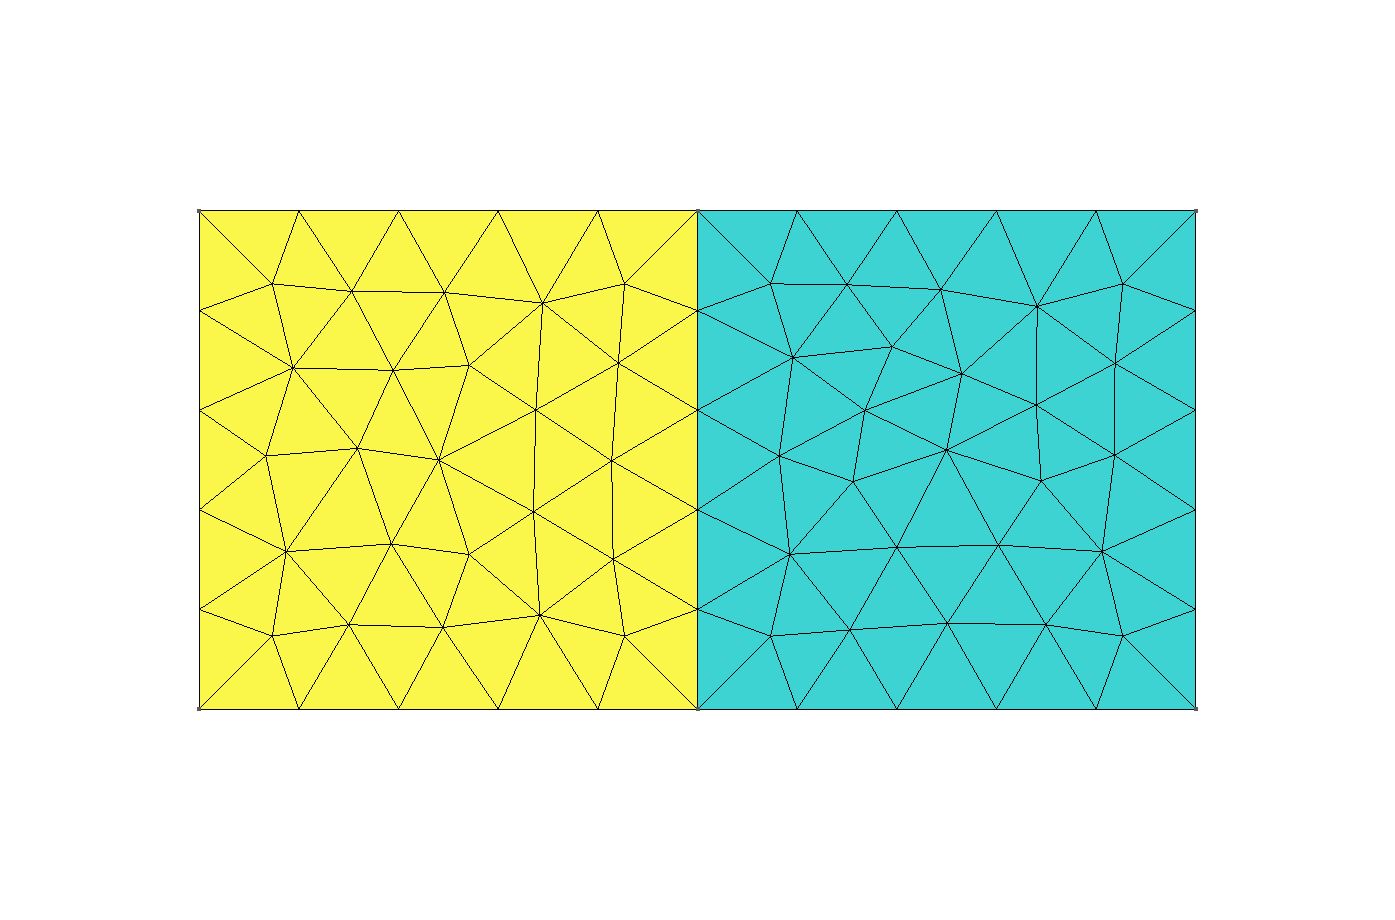
\includegraphics{design/parametric/two-squares-triang.png}\label{fig:two-squares-triang}}

\subfloat[Quadrangles]{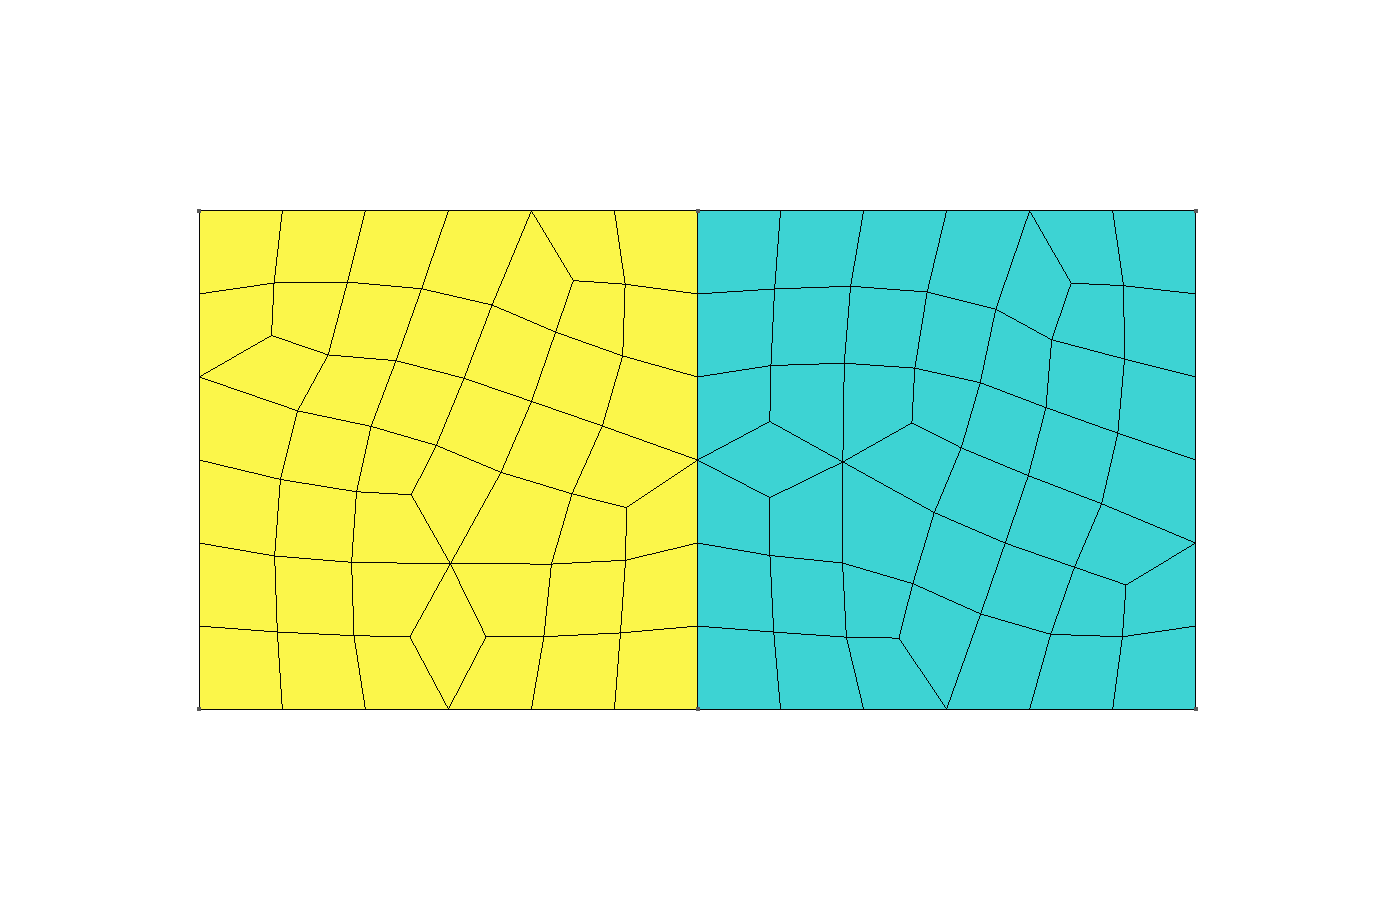
\includegraphics{design/parametric/two-squares-quad.png}\label{fig:two-squares-quad}}

\caption{Heat conduction on two 2D squares with different
temprature-depedent conductivities}

\label{fig:two-squares}

\end{figure}

\begin{lstlisting}[style=feenox]
READ_MESH two-squares-$2.msh DIMENSIONS 2
PROBLEM thermal

# per-material conductivity
k_soft(x,y) := 1+T(x,y)
k_hard(x,y) := 1-0.1*T(x,y)

BC left  T=0
BC right T=$1

SOLVE_PROBLEM
PRINT TEXT $1 TEXT "Tright=$1" T(1,0.5)
\end{lstlisting}

\noindent and the shell script

\begin{lstlisting}[language=bash, style={bash.sh}]
for temp in $(seq 1 3); do
 for shape in triang quad; do
   feenox two-squares-thermal.fee ${temp} ${shape}
 done
done
\end{lstlisting}

Then it is possible to run the six combinations at once, obtaining

\begin{lstlisting}
$ ./two-squares-thermal.sh
1       Tright=1        0.432843
1       Tright=1        0.432965
2       Tright=2        0.767466
2       Tright=2        0.767729
3       Tright=3        1.03429
3       Tright=3        1.03464
\end{lstlisting}

This way of performing parametric studies is very flexible since the
varied arguments can be either strings or numbers. Both the actual input
itself and the external driver script can be tracked using version
control systems, allowing for an efficient and flexible traceability
scheme. This is a design feature of FeenoX, inspired by the UNIX rules
of generation and of economy.

The second way of running parametric studies is by using the internal
keyword \passthrough{\lstinline!PARAMETRIC!} that allows sweeping a
numerical range of one or more FeenoX variables.

\textbf{TODO}

\hypertarget{sec:efficiency}{%
\subsection{Efficiency}\label{sec:efficiency}}

\begin{quote}
The computational resources (i.e.~costs measured in CPU/GPU time,
random-access memory, long-term storage, etc.) needed to solve a problem
should be comparable to other similar state-of-the-art finite-element
tools.
\end{quote}

\begin{quote}
The computational resources (i.e.~costs measured in CPU/GPU time,
random-access memory, long-term storage, etc.) needed to solve a problem
should be comparable to other similar state-of-the-art finite-element
tools.
\end{quote}

cloud, rent don't buy benchmark and comparisons

\hypertarget{sec:scalability}{%
\subsection{Scalability}\label{sec:scalability}}

\begin{quote}
The tool ought to be able to start solving small problems first to check
the inputs and outputs behave as expected and then allow increasing the
problem size up in order to achieve to the desired accuracy of the
results. As mentioned in sec.~\ref{sec:architecture}, large problem
should be split among different computers to be able to solve them using
a finite amount of per-host computational power (RAM and CPU).
\end{quote}

PETSc, MPI error handling, rule of repair check all malloc() calls

\hypertarget{flexibility}{%
\subsection{Flexibility}\label{flexibility}}

\begin{quote}
The tool should be able to handle engineering problems involving
different materials with potential spatial and time-dependent
properties, such as temperature-dependent thermal expansion coefficients
and/or non-constant densities. Boundary conditions must be allowed to
depend on both space and time as well, like non-uniform pressure loads
and/or transient heat fluxes.
\end{quote}

FeenoX comes from nuclear + experience (what to do and what not to do)

Materials: a material library (perhaps included in a frontend GUI?) can
write FeenoX' material definitions. Flexiblity.

\hypertarget{sec:extensibility}{%
\subsection{Extensibility}\label{sec:extensibility}}

\begin{quote}
It should be possible to add other PDE-casted problem types (such as the
Schröedinger equation) to the tool using a reasonable amount of time by
one or more skilled programmers. The tool should also allow new models
(such as non-linear stress-strain constitutive relationships) to be
added as well.
\end{quote}

user-provided routines skel for pdes and annotated models

\hypertarget{sec:interoperability}{%
\subsection{Interoperability}\label{sec:interoperability}}

\begin{quote}
A mean of exchanging data with other computational tools complying to
requirements similar to the ones outlined in this document.
\end{quote}

UNIX POSIX

\hypertarget{interfaces}{%
\section{Interfaces}\label{interfaces}}

\begin{quote}
The tool should be able to allow remote execution without any user
intervention after the tool is launched. The problem should be
completely defined in one or more input files and the output should be
complete and useful after the tool finishes its execution as in
fig.~\ref{fig:transfer}.

The tool should be able to report the status of the execution
(i.e.~progress, errors, etc.) and to make this information available to
the user or process that launched the execution, possibly from a remote
location.
\end{quote}

\hypertarget{sec:input}{%
\subsection{Problem input}\label{sec:input}}

\begin{quote}
No GUI. Plain ASCII input file and/or interpreted high-level language
API. Mobile \& web-friendly.

\textbf{Simple problems should need simple inputs.}

\textbf{Similar problems should need similar inputs.}

VCS tracking

These input files might be

\begin{itemize}
\tightlist
\item
  particularly formatted files to be read by the tool in an
  \emph{ad-hoc} way, and/or
\item
  source files for interpreted languages which can call the tool through
  and API or equivalent method, and/or
\item
  any other method that can fulfill the requirement illustrated
  in~fig.~\ref{fig:transfer}
\end{itemize}
\end{quote}

dar ejemplos comparar con
\url{https://cofea.readthedocs.io/en/latest/benchmarks/004-eliptic-membrane/tested-codes.html}

macro-friendly inputs, rule of generation

\hypertarget{sec:output}{%
\subsection{Results output}\label{sec:output}}

\begin{quote}
Output should not be cluttered up with non-mandatory information. Time
of cognizant engineers should be more important than time needed for
computation. JSON/YAML, state of the art open post-processing formats.
Mobile \& web-friendly.

Common and preferably open-source formats.
\end{quote}

100\% user-defined output with PRINT, rule of silence rule of economy,
i.e.~no RELAP yaml/json friendly outputs vtk (vtu), gmsh

\hypertarget{sec:qa}{%
\section{Quality assurance}\label{sec:qa}}

\begin{quote}
Since the results obtained with the tools might be used in verifying
existing equipment or in designing new mechanical parts in sensitive
industries, a certain level of software quality assurance is needed.
Some best-practices for developing generic software as required, such as
employment of a version control system, automated unit testing and bug
tracking support. But also more particular verification and validation
procedures for the particular case of engineering computational software
is
\end{quote}

\hypertarget{reproducibility-and-traceability}{%
\subsection{Reproducibility and
traceability}\label{reproducibility-and-traceability}}

\begin{quote}
The full source code and the documentation of the tool ought to be
maintained under a control version system hosted on a public server
accessible worldwide without needing any special credentials to get a
copy of the code.

All the information needed to solve a particular problem (i.e.~meshes,
boundary conditions, spatially-distributed material properties, etc.)
should be generated from a very simple set of files which ought to be
susceptible of being tracked with current state-of-the-art version
control systems.

simple \textless-\textgreater{} simple

similar \textless-\textgreater{} similar

Mesh data should be mixed with the problem data like material properties
or boundary conditions. Changes in the mesh should be tracked on the
files needed to create the mesh and not on the mesh itself.
\end{quote}

\hypertarget{automated-testing}{%
\subsection{Automated testing}\label{automated-testing}}

\begin{quote}
A mean to automatically test the code for regressions is mandatory. A
set of problems with known solutions should be solved with the tool
after each modification of the code to make sure these changes still
give the right answers for the right questions. Unit software testing
practices like continuous integration are recommended.
\end{quote}

\hypertarget{bug-reporting-and-tracking}{%
\subsection{Bug reporting and
tracking}\label{bug-reporting-and-tracking}}

\begin{quote}
A system to allow developers and users to report errors, bugs and
improvements should be provided. If applicable, these reports should be
tracked, addressed and documented.
\end{quote}

\hypertarget{sec:verification}{%
\subsection{Verification}\label{sec:verification}}

\begin{quote}
The source code should be available for verification by independent
third parties. Changes in the source code should be controllable,
traceable and well documented. Stable releases ought to be digitally
signed by a responsible engineer.
\end{quote}

open source (really, not like CCX -\textgreater{} mostrar ejemplo)
GPLv3+ free Git + gitlab, github, bitbucket

\hypertarget{validation}{%
\subsection{Validation}\label{validation}}

\begin{quote}
The tool should be verified against known analytical results and other
already-validated tools according to existing industry standards such as
ASME or IAEA.
\end{quote}

\hypertarget{sec:documentation}{%
\subsection{Documentation}\label{sec:documentation}}

\begin{quote}
Documentation should be complete and cover both the user and the
developer point of view. It should contain a user manual adequate for
both reference and tutorial purposes. Other forms of simplified
documentation such as quick reference cards or video tutorials are not
mandatory but highly recommended. Since the tool should be extendable
(sec.~\ref{sec:extensibility}), there should be a separate development
manual covering the programming design and implementation and how to
extend and add new features. Also, as non-trivial mathematics which
should be verified (sec.~\ref{sec:verification}) are expected, an
explanation what equations are taken into account and how they are
solved is required.

It should be possible to make the full documentation available online in
a way that it can be both printed in hard copy and accessed easily from
a mobile device. Users modifying the tool to suit their own needs should
be able to modify the associated documentation as well.
\end{quote}

it's not compact, but almost! Compactness is the property that a design
can fit inside a human being's head. A good practical test for
compactness is this: Does an experienced user normally need a manual? If
not, then the design (or at least the subset of it that covers normal
use) is compact. unix man page markdown + pandoc = html, pdf, texinfo

\hypertarget{sec:unix}{%
\section{Appendix: Rules of UNIX philosophy}\label{sec:unix}}

\begin{description}
\item[Rule of Modularity]
Developers should build a program out of simple parts connected by well
defined interfaces, so problems are local, and parts of the program can
be replaced in future versions to support new features. This rule aims
to save time on debugging code that is complex, long, and unreadable.

\emph{In FeenoX:} there are some skels that show how new problems can be
added (i.e.~replace the thermal equations with electromagnetism)
\item[Rule of Clarity]
Developers should write programs as if the most important communication
is to the developer who will read and maintain the program, rather than
the computer. This rule aims to make code as readable and comprehensible
as possible for whoever works on the code in the future.

\emph{In FeenoX:} we attempt to do that, not sure if we nail it\ldots{}
\item[Rule of Composition]
Developers should write programs that can communicate easily with other
programs. This rule aims to allow developers to break down projects into
small, simple programs rather than overly complex monolithic programs.

\emph{In FeenoX:} this is FeenoX' main point, to use a mesh created by
another tool and to create files which can be post-processed by other
tools. Other that these files which have a definite format, the output
of the program is 100\% controlled by the user so it can be tailored to
suit any other programs' input needs.
\item[Rule of Separation]
Developers should separate the mechanisms of the programs from the
policies of the programs; one method is to divide a program into a
front-end interface and a back-end engine with which that interface
communicates. This rule aims to prevent bug introduction by allowing
policies to be changed with minimum likelihood of destabilizing
operational mechanisms.

\emph{In FeenoX:} this is related to the previous rule, separation is
the basic idea of FeenoX.
\item[Rule of Simplicity]
Developers should design for simplicity by looking for ways to break up
program systems into small, straightforward cooperating pieces. This
rule aims to discourage developers' affection for writing ``intricate
and beautiful complexities'' that are in reality bug prone programs.

\emph{In FeenoX:} we attempt to do that, not sure if we nail it\ldots{}
\item[Rule of Parsimony]
Developers should avoid writing big programs. This rule aims to prevent
overinvestment of development time in failed or suboptimal approaches
caused by the owners of the program's reluctance to throw away visibly
large pieces of work. Smaller programs are not only easier to write,
optimize, and maintain; they are easier to delete when deprecated.

\emph{In FeenoX:} we attempt to do that, not sure if we nail it\ldots{}
\item[Rule of Transparency]
Developers should design for visibility and discoverability by writing
in a way that their thought process can lucidly be seen by future
developers working on the project and using input and output formats
that make it easy to identify valid input and correct output. This rule
aims to reduce debugging time and extend the lifespan of programs.

\emph{In FeenoX:} we attempt to do that, not sure if we nail it\ldots{}
\item[Rule of Robustness]
Developers should design robust programs by designing for transparency
and discoverability, because code that is easy to understand is easier
to stress test for unexpected conditions that may not be foreseeable in
complex programs. This rule aims to help developers build robust,
reliable products.

\emph{In FeenoX:} we attempt to do that, not sure if we nail it\ldots{}
\item[Rule of Representation]
Developers should choose to make data more complicated rather than the
procedural logic of the program when faced with the choice, because it
is easier for humans to understand complex data compared with complex
logic. This rule aims to make programs more readable for any developer
working on the project, which allows the program to be maintained.

\emph{In FeenoX:} that's why we use C instead of Fortran. And in some
way, that's also why we use C instead of C++. But it might depend on who
the developer working on the project is and what background she
has\ldots{}
\item[Rule of Least Surprise]
Developers should design programs that build on top of the potential
users' expected knowledge; for example, `+' in a calculator program
should always mean `addition'. This rule aims to encourage developers to
build intuitive products that are easy to use.

\emph{In FeenoX:} a `+' in FeenoX means addition, etc. The input file
looks like a near-English text that actually works like a
syntactically-sugared set of instructions that teels FeenoX how to solve
a problem.
\item[Rule of Silence]
Developers should design programs so that they do not print unnecessary
output. This rule aims to allow other programs and developers to pick
out the information they need from a program's output without having to
parse verbosity.

\emph{In FeenoX:} if there are not explicit
\passthrough{\lstinline!PRINT!} instructions, FeenoX does not write
anythin to the standard output. Actually, without any explicit
\passthrough{\lstinline!WRITE!} instruction, no output files would be
written either.
\item[Rule of Repair]
Developers should design programs that fail in a manner that is easy to
localize and diagnose or in other words ``fail noisily''. This rule aims
to prevent incorrect output from a program from becoming an input and
corrupting the output of other code undetected.

\emph{In FeenoX:} input errors are detected before the computation is
started and run-time errors (i.e.~a division by zero) con be user
controled, they can be fatal or ignored.
\item[Rule of Economy]
Developers should value developer time over machine time, because
machine cycles today are relatively inexpensive compared to prices in
the 1970s. This rule aims to reduce development costs of projects.

\emph{In FeenoX:} related to rule of silence, FeenoX will write only
what the user asks for in order to save her from parsing through tons of
undesired data. The approach of ``compute and write everything you can
in one single run'' made sense in 1970 where CPU time was expensive, but
not anymore.
\item[Rule of Generation]
Developers should avoid writing code by hand and instead write abstract
high-level programs that generate code. This rule aims to reduce human
errors and save time.

\emph{In FeenoX:} not so much for code but definitely for documentation.
\item[Rule of Optimization]
Developers should prototype software before polishing it. This rule aims
to prevent developers from spending too much time for marginal gains.

\emph{In FeenoX:} we are still building, we'll optimize later.
\item[Rule of Diversity]
Developers should design their programs to be flexible and open. This
rule aims to make programs flexible, allowing them to be used in ways
other than those their developers intended.

\emph{In FeenoX:} unexpected usage happens more than often. Flexiblity
is a key cornerstone.
\item[Rule of Extensibility]
Developers should design for the future by making their protocols
extensible, allowing for easy plugins without modification to the
program's architecture by other developers, noting the version of the
program, and more. This rule aims to extend the lifespan and enhance the
utility of the code the developer writes.

\emph{In FeenoX:} open source code and GPL license encourages
extensions.
\end{description}

\end{document}
